\documentclass[12pt]{article}
\usepackage[margin=1in]{geometry}
\usepackage{graphicx}
\usepackage{float}
\usepackage{caption}
\usepackage{subcaption}
\usepackage{amsmath}
\usepackage{amsfonts}
\usepackage{amssymb}
\usepackage{listings}
\usepackage{color}
\usepackage{xcolor}

\lstset{
    language=C, % Embedded C is based on C
    basicstyle=\ttfamily\small, % Monospace font
    keywordstyle=\color{blue}, % Keywords in blue
    commentstyle=\color{gray}, % Comments in gray
    stringstyle=\color{red}, % Strings in red
    numbers=left, % Line numbers on the left
    numberstyle=\tiny\color{gray}, % Style of line numbers
    stepnumber=1, % Number every line
    breaklines=true, % Wrap long lines
    frame=single, % Frame around the code block
    captionpos=b, % Caption position below the listing
    tabsize=4, % Tab spacing
}

\title{\textbf{Scientific Calculator}}
\author{\textbf{John Bobby}\\ \textbf{ee24btech11032}}
\date{}
\begin{document}
\maketitle
\section{Objective}
The objective of this project is to design and implement a scientific calculator using an Arduino and push buttons. The calculator will be capable of performing basic arithmetic operations as well as evaluating trigonometric functions and their inverses. The implementation will be done using Embedded C.

\section{Hardware Components}
\begin{itemize}
    \item Arduino
    \item $16 \times 2$LCD display
    \item 14 push buttons
    \item 10K potentiometer
    \item Jumper Wires
\end{itemize}
\begin{figure}[H]
    \centering
    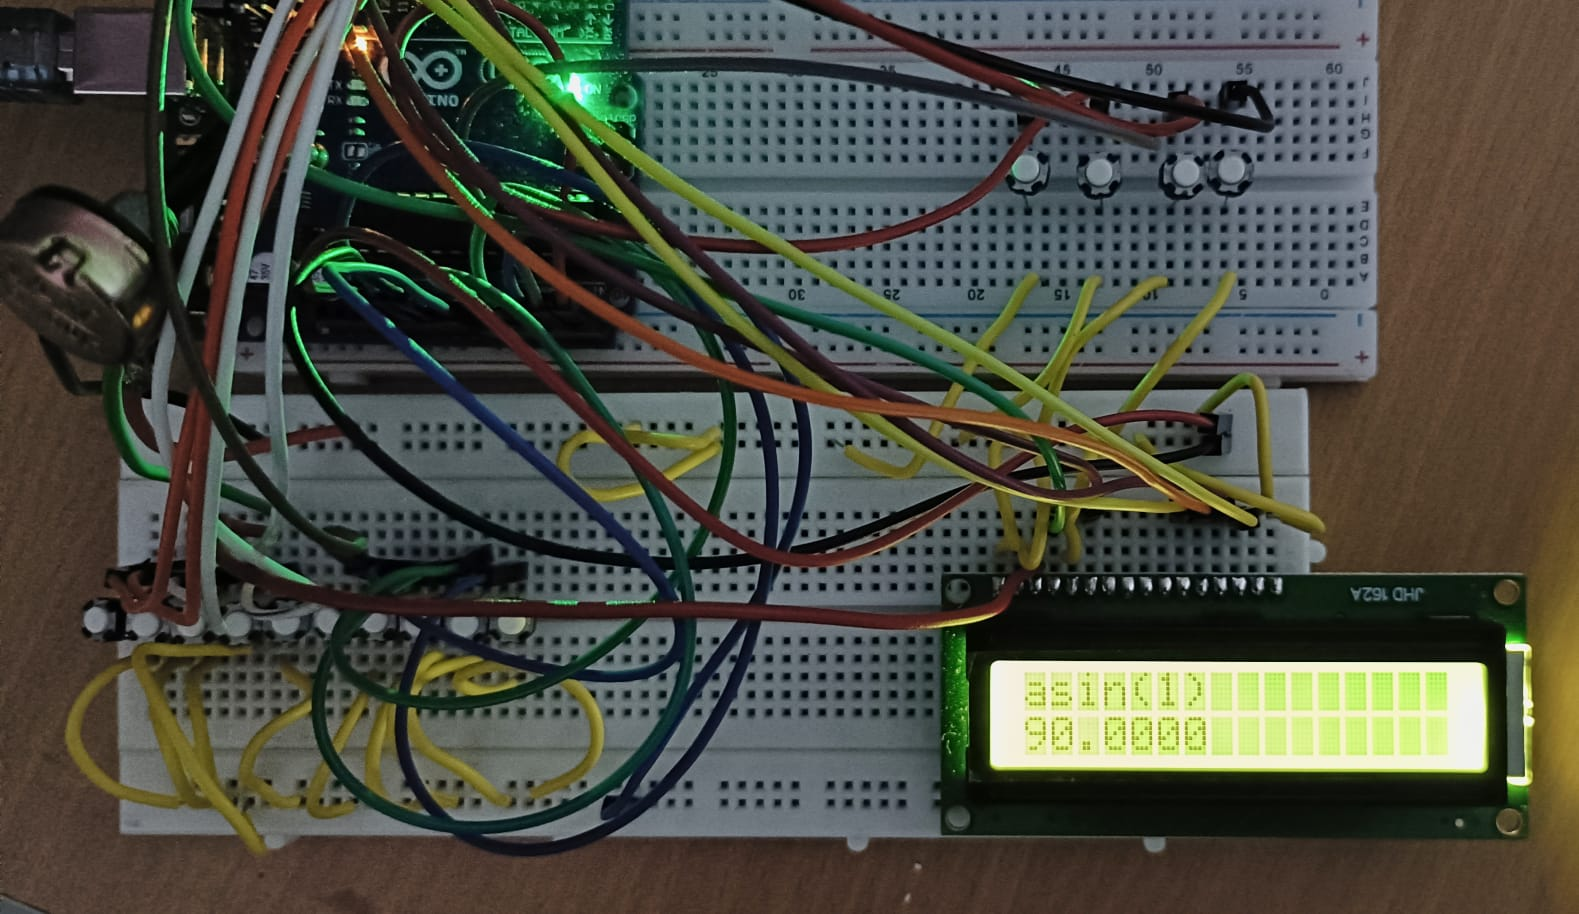
\includegraphics[width=0.8\linewidth]{fig1.jpg}
    \caption{Calculator}
    \label{fig:enter-label}
\end{figure}
 \section{Connections}
 \begin{table}[H]
     \centering
        \begin{tabular}{|c|c|}  % Adjust columns as needed
        \hline
        \textbf{Pin(Arduino)} & \textbf{Connected To} \\  % Header row
        \hline
        2,3,4,5 & A,B,C,D of 7447 IC \\  
        \hline
        6,7,8,9,10,11 & COM of all the 6 displays  \\ 
        \hline
        5V, GND & $V_{cc}$ and GND of 7447 IC  \\  
        \hline
    \end{tabular}

     \caption{Connections}
     \label{tab:my_label}
 \end{table}

 \section{Button Implementation and Detection}


\subsection{Button Circuit and Pin Configuration}
\begin{itemize}
    \item When the button is NOT pressed, the input reads HIGH due to the \textbf{internal pull-up} resistor.
    \item When the button is pressed, it connects to ground GND, and the input reads LOW.
\end{itemize}
This helps prevent floating states and ensures stable detection of button presses.

\subsection{Debounce Logic for Button Presses}

When we press a button, mechanical vibrations of the metal parts may give false reading.
\begin{itemize}
    \item Read the button state (HIGH or LOW).
    \item If the state remains stable for a predefined debounce time (50 ms), confirm the button press.
\end{itemize}
\section{ Button Debounce in Code}
\begin{lstlisting}[caption={Deboune Logic}, label={lst:multiplexing}]
uint8_t read_button(Button *b) {
    if ((*(b->pin) & (1 << b->bit)) == 0) {  // Button pressed (active low)
        _delay_ms(DEBOUNCE_DELAY_MS);        // Wait for debounce period
        if ((*(b->pin) & (1 << b->bit)) == 0) {  // Check if still pressed
            return 1;
        }
    }
    return 0;
}
\end{lstlisting}
\begin{itemize}
    \item Checks if the button is pressed before and after the debounce time.
\end{itemize}
\section{Digit Handling}
\begin{lstlisting}[caption={Digit Handling Logic}, label={lst:multiplexing}]
if (read_button(&digitButtons[i])) {
    uint8_t digit = i;
    if (!decimalEntered) {
        currentNumber = currentNumber * 10 + digit;
    } else {
        currentNumber = currentNumber + digit * decimalMultiplier;
        decimalMultiplier *= 0.1;
    }
    append_digit(digit);
    lcd_clear();
    lcd_print(displayStr);
}
\end{lstlisting}
\begin{itemize}
    \item A variable called decimalEntered is created which is True when we press the decimal point button.
    \item currentNumber variable is updated accordingly.
    \item All operations are handled with the help of if statements.
\end{itemize}
\section{Conclusion}


One of the key challenges in this project was ensuring \textbf{accurate button press detection}, which was efficiently handled using \textbf{debouncing techniques}.

Overall, this project demonstrates the feasibility of implementing a \textbf{low-cost, efficient, and user-friendly} calculator using microcontrollers. Future improvements could include \textbf{touch-based input}, \textbf{floating-point optimization}, or even \textbf{integration with external memory} to store previous calculations. This project not only reinforces fundamental concepts of \textbf{embedded systems} but also provides a foundation for more advanced digital electronics applications.







\end{document}

